\section{Introduzione}

\subsection{Definizioni fondamentali}

La \textit{data inference} è lo studio dei metodi che utilizzano i dati per predirre il futuro. 
Il \textit{Machine Learning} è uno strumento potente che può essere usato per risolvere una 
grossa parte dei problemi di \textit{data inference}, inclusi i seguenti:
\begin{itemize}
    \item \textbf{Clustering}: raggruppare i \textit{data points} in base alle loro similarità;
    \item \textbf{Prediction}: assegnare delle etichette (\textit{label}) ai \textit{data points};
    \item \textbf{Generation}: generare nuovi \textit{data points};
    \item    \textbf{Control}: eseguire una sequenza di azioni in un ambiente con l'obiettivo di
                               massimizzare una nozione di utilità.
\end{itemize}

Con \textit{data point} si intende una serie di informazioni legate ad un unico elemento;
un'analogia può essere un \textit{record} in un database.

Gli algoritmi che risolvono una \textit{learning task} in base a dei dati già semanticamente
etichettati lavorano in modalità \textbf{\textit{supervised learning}}. A etichettare i dati
saranno delle persone o la natura. Un esempio dell'ultimo caso sono le previsioni del meteo. 
D'altra parte, gli algoritmi che utilizzano i dati senza la presenza di etichette lavorano in
modalità \textbf{\textit{unsupervised learning}}.

In questo corso ci si focalizzerà sul \textit{supervised learning} e la progettazione di 
sistemi di \textit{machine learning} il cui obiettivo è apprendere dei 
\textbf{predittori}, ovvero funzioni che mappano i \textit{data points} alla loro
etichetta.

\subsubsection{\textit{Label set} \texorpdfstring{$\Y$}{Y}}
Verrà usata $\Y$ per indicare il \textit{label set}, ovvero l'insieme di tutte le possibili
etichette di un \textit{data point}. Le etichette potranno essere di due tipi differenti:
\begin{enumerate}
    \item \textbf{Categoriche} ($\Y = \{ \text{sport},\text{politica},\text{economia}\}$):
        si parlerà di problemi di \textbf{classificazione};
    \item \textbf{Numeriche} ($\Y \subseteq \RN $): 
        si parlerà di problemi di \textbf{regressione}.
\end{enumerate}

È importante sottolineare come la reale differenza tra le due tipologie di etichetta sia il
significato e non la sua rappresentazione in quanto, si potrà sempre codificare
un'etichetta categorica in un numero.

A sottolineare ciò è il fatto che nella regressione l'errore è tipicamente una funzione della
differenza $| y-\hat{y} |$, dove $\hat{y}$ è la predizione di $y$. Nella classificazione, invece,
l'errore è tipicamente binario: predizione corretta ($\hat{y}=y$) o errata ($\hat{y}\neq y$).

Quando ci sono solo due possibili etichette ($|\Y|=2$), si ha un \textbf{problema di 
classificazione binario} e, convenzionalmente, verrà usata una codifica numerica 
$\Y=\{-1,1\}$.

\subsubsection{\textit{Loss function} \texorpdfstring{$\loss$}{l}}
Come già visto precedentemente, si vuole misurare l'errore che un predittore commette su una
determinata predizione. Per farlo si userà una \textbf{funzione di loss} $\loss$ non negativa 
che misurerà la discrepanza $\loss(y,\hat{y})$ tra l'etichetta predetta $\hat{y}$ e quella
corretta $y$. Si assumerà sempre $\loss(y,\hat{y})=0$ quando $\hat{y}=y$.

La funzione di loss più semplice per la classificazione è la \textbf{zero-one loss}:
$$ \loss(y,\hat{y}) = \begin{cases} 0 & y=\hat{y} \\ 1 & \text{altrimenti} \end{cases} $$

Nella regressione, le tipiche funzioni di loss sono:
\begin{itemize}
    \item la \textit{\textbf{absolute loss}}: $\loss(y,\hat{y}) = |y-\hat{y}|$
    \item la \textit{\textbf{quadratic loss}}: $\loss(y,\hat{y}) = (y-\hat{y})^2$
\end{itemize}

In alcuni casi può essere conveniente scegliere l'etichetta predetta da un insieme $\Z$ diverso 
da $\Y$. Per esempio, si consideri il problema di assegnare una probabilità $\hat{y}\in (0,1)$
all'evento $y=\text{\quotes{pioverà domani}}$. In questo caso, $\Y=\{\text{\quotes{piove}},
\text{\quotes{non piove}}\}$ e $\Z = (0,1)$. Indicando questi due eventi con 1 (piove) e 0 
(non piove), si può usare una funzione di loss per la regressione, come la 
\textit{absolute loss}:
$$ \loss(y,\hat{y}) = |y-\hat{y}| =  \begin{cases} 1-\hat{y} & y=1 \qquad (\text{piove}) \\
\hat{y} & y=0 \qquad (\text{non piove}) \end{cases} $$

Per penalizzare maggiormente le predizioni che distano troppo dalla realtà, si può usare una
\textit{\textbf{logarithmic loss}}:
$$ \loss(y,\hat{y}) = \begin{cases} \ln{\frac{1}{\hat{y}}} & y=1 \qquad 
(\text{piove}) \\ \ln{\frac{1}{1-\hat{y}}} & y=0 \qquad (\text{non piove}) \end{cases} $$

\begin{figure}[h]
    \centering
    \begin{subfigure}{.43\textwidth}
        \centering
        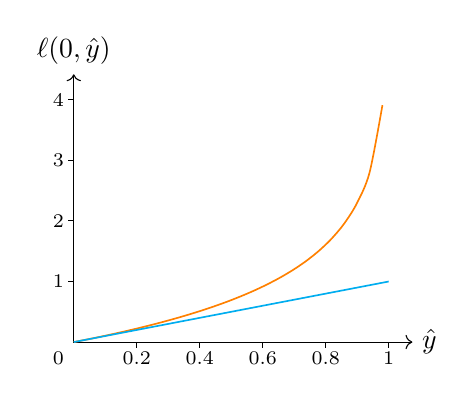
\begin{tikzpicture}

    \draw[<->] (4.3,0) node[right]{$\hat{y}$} -|(0,3.4) node[above]{$\ell(0,\hat{y})$};
    \draw[domain=0:0.98, semithick, smooth, orange] plot ({\x*4},{ln(1/(1-\x))/1.3});
    \draw[domain=0:1, semithick, cyan] plot ({\x*4},{abs(0-\x)/1.3});

    \node[below left] at (0,0) {\scriptsize 0};
    %xticks
    \foreach \x in {0.2,0.4,...,1} {
        \draw (\x*4,0) -- (\x*4,-.07);
    }
    \node[below] at (0.2*4,0) {\scriptsize 0.2};
    \node[below] at (0.4*4,0) {\scriptsize 0.4};
    \node[below] at (0.6*4,0) {\scriptsize 0.6};
    \node[below] at (0.8*4,0) {\scriptsize 0.8};
    \node[below] at (1*4,0)   {\scriptsize 1};
    %yticks
    \foreach \y in {1,...,4} {
        \draw (0,\y/1.3) -- (-.07,\y/1.3);
    }
    \node[left] at (0,1/1.3) {\scriptsize 1};
    \node[left] at (0,2/1.3) {\scriptsize 2};
    \node[left] at (0,3/1.3) {\scriptsize 3};
    \node[left] at (0,4/1.3) {\scriptsize 4};

\end{tikzpicture}
    \end{subfigure}
    \begin{subfigure}{.43\textwidth}
        \centering
        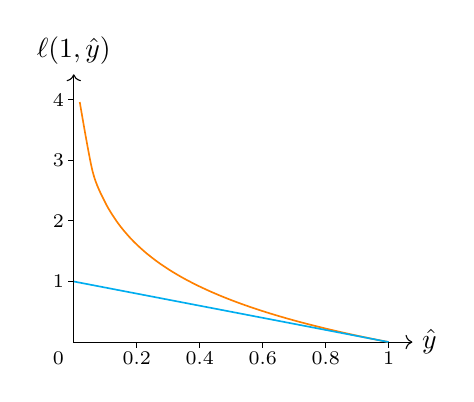
\begin{tikzpicture}

    \draw[<->] (4.3,0) node[right]{$\hat{y}$} -|(0,3.4) node[above]{$\ell(1,\hat{y})$};
    \draw[domain=0.019:1, semithick, smooth, orange] plot ({\x*4},{ln(1/\x)/1.3});
    \draw[domain=0:1, semithick, cyan] plot ({\x*4},{abs(1-\x)/1.3});

    \node[below left] at (0,0) {\scriptsize 0};
    %xticks
    \foreach \x in {0.2,0.4,...,1} {
        \draw (\x*4,0) -- (\x*4,-.07);
    }
    \node[below] at (0.2*4,0) {\scriptsize 0.2};
    \node[below] at (0.4*4,0) {\scriptsize 0.4};
    \node[below] at (0.6*4,0) {\scriptsize 0.6};
    \node[below] at (0.8*4,0) {\scriptsize 0.8};
    \node[below] at (1*4,0)   {\scriptsize 1};
    %yticks
    \foreach \y in {1,...,4} {
        \draw (0,\y/1.3) -- (-.07,\y/1.3);
    }
    \node[left] at (0,1/1.3) {\scriptsize 1};
    \node[left] at (0,2/1.3) {\scriptsize 2};
    \node[left] at (0,3/1.3) {\scriptsize 3};
    \node[left] at (0,4/1.3) {\scriptsize 4};

\end{tikzpicture}
    \end{subfigure}
    \caption{Confronto tra \textit{\color{cyan}absolute loss} e \textit{\color{orange}
    logarithmic loss}; a sinistra il caso $y=0$, a destra $y=1$. \label{fig:abs_vs_log}}
\end{figure}

Si noti in figura \ref{fig:abs_vs_log} come la \textit{logarithmic loss} tenda ad
infinito quando la predizione è opposta all'etichetta reale:
$$\lim_{\hat{y}\rightarrow 1^-} \loss(0,\hat{y})=\lim_{\hat{y}\rightarrow 0^+}
\loss(1,\hat{y}) = +\infty$$
In pratica questo previene 
l'utilizzo di predizioni $\hat{y}$ troppo sicure, quindi troppo vicine a zero o uno.

\subsubsection{\textit{Data domain} \texorpdfstring{$\X$}{X}}
Verrà usata $\X$ per indicare l'insieme dei \textit{data points}; ogni suo punto $x \in \X$
è tipicamente un record di un database formato da \textit{feature}:
$$ x = (x_1, \dots , x_d) $$
Spesso un \textit{data point} può essere codificato come un vettore i cui elementi sono le
sue \textit{feature}. Questa codifica risulta naturale in presenza di quantità omogenee, come
i pixel di un'immagine o una lista di occorrenze di parole in un testo. Quando invece i dati
presenti utilizzano unità di misura differenti, come \quotes{età} e \quotes{altezza}, la
codifica non risulta più immediata. Ci sarà bisogno di una procedura che codifichi i dati
in modo da ottenere uno spazio vettoriale omogeneo e coerente con i dati iniziali.

In questo corso si assumerà che i dati possano essere rappresentati da vettori di numeri:
$$ \X \equiv \RN^d $$

\subsubsection{Predittori \texorpdfstring{$f$}{f}}

Un \textbf{predittore} è una funzione $\pred:\X \rightarrow \Y$ che mappa i
\textit{data points} alle etichette (o $\pred:\X \rightarrow \Z$). Sì può quindi
dire che in un problema di predizione l'obiettivo è ottenere una funzione $\pred$ 
che genera delle predizioni $\hat{y} = \pred(x)$ tali che $\loss(y,\hat{y})$ sia
basso per il maggior numero di punti $x \in \X$ osservati. In pratica, \textbf{la 
funzione $\pred$ è definita da un certo numero di parametri in un dato modello}. Un
esempio sono i parametri di una rete neurale.

\subsubsection{Esempi}
Nel \textit{supervised learning} un \textbf{esempio} è una coppia $(x,y)$ dove $x$
è un \textit{data point} e $y$ la sua reale etichetta.

In alcuni casi $x$ ha un'unica $y$, come nel caso in cui $y$ rappresenta una proprietà
oggettiva di $x$; in altri casi, invece, $x$ può avere diverse $y$ associate, come
quando le $y$ sono soggettivamente assegnate da persone.

\subsubsection{\textit{Test set} e \textit{test error}}
Per poter stimare la qualità di un predittore si usa un insieme di esempi detto
\textbf{\textit{test set}}:
$$ \{ (x_1',y_1'),\dots, (x_n',y_n')\} $$
Data una \textit{loss function} $\loss$, il \textit{test set} viene usato per
calcolare il \textit{\textbf{test error}} di un predittore $\pred$:
$$ \frac{1}{n}\sum^{n}_{t=1}{
    \loss(\underbrace{y_t'}_{\mathclap{\text{reale}}},
    \overbrace{\pred(x_t')}^{\mathclap{\text{predetta}}})} $$

Il \textit{test error} ha quindi lo scopo di calcolare la prestazione media del 
predittore su dei dati reali.

\subsubsection{\textit{Learning algorithm} \texorpdfstring{$A$}{A}}
Si definisce \textit{training set} $S$ un insieme di esempi:
$$ S = \{(x_1,y_1),\dots,(x_m,y_m)\} $$
che viene usato dal \textbf{\textit{learning algorithm} $A$} per produrre un predittore
$A(S)$.
Informalmente, il \textit{learning algorithm} \quotes{impara} dal \textit{training set}.

\vspace{1em}

\begin{figure}[h]
    \centering
    \usetikzlibrary {arrows.meta} 
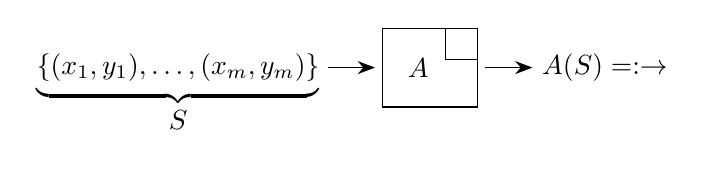
\begin{tikzpicture}

    \node at (0.4,1.5) {$\{(x_1,y_1),\dots,(x_m,y_m)\}$};
    \node at (0.4,1.15) {$\underbrace{\phantom{\{(x_1,y_1),\dots,(x_m,y_m)\}}}_{\displaystyle S}$};
    \draw[-{Stealth[length=2.2mm]}] (2.3,1.5) -- (2.9,1.5);
    \draw (3,2) rectangle (4.2,1);
    \node at (3.45,1.5) {$A$};
    \draw (3.8,2) rectangle (4.2,1.6) node[pos=.5] {$\loss$};
    \draw[-{Stealth[length=2.2mm]}] (4.3,1.5) -- (4.9,1.5)
        node [right] {$A(S) = \pred: \X \rightarrow \Y$};

\end{tikzpicture}
\end{figure}

Il \textit{test set} e il \textit{training set} vengono solitamente prodotti assieme
attraverso un processo di collezione dati e etichettamento. Dato l'insieme di esempi
preparati, questo verrà partizionato in \textit{test set} e \textit{training set},
tipicamente tramite una divisione casuale. \textbf{Obiettivo del corso è lo sviluppo
di una teoria che ci guidi nella progettazione di \textit{learning algorithm} che
generano predittori con un basso \textit{test error}}.

\subsubsection{\textit{Training error} \texorpdfstring{$\loss_S$}{l}}
Sia $S = \{(x_1,y_1),\dots,(x_m,y_m)\}$ il \textit{training set}; viene definito,
equivalentemente al \textit{test error}, il \textbf{\textit{training error}}:
$$ \loss_S(\pred) = \frac{1}{m}\sum_{t=1}^m \loss(y_t,\pred(x_t)) $$

\textbf{Un approccio intuitivo alla progettazione di \textit{learning algorithm} è 
quello di assumere che il \textit{training error} $\loss_S(\pred)$ del predittore 
$\pred$ sia correlato con il suo \textit{test error}}.

\subsection{Empirical Risk Minimization (ERM)}

\subsubsection{Definizione}
Sia $\F$ un insieme di predittori e $\loss$ una \textit{loss function}.
L'\textit{empirical risk minimizer} (ERM) è il \textit{learning algorithm} $A$
che restituisce un predittore in $\F$ che \textbf{minimizza il 
\textit{training error}}:
$$ A(S) \in \argmin_{f \in \F} \loss_S(f) $$

Si noti come $A(S)$ appartenga e non uguagli il minimo; questo perchè ci 
potrebbero essere più $f \in \F$ che minimizzano $\loss_S(f)$.

\subsubsection{Predittori con \textit{test error} elevato}
Quando in $\F$ tutti i predittori hanno un \textit{test error} alto, ERM produrrà
un pessimo predittore. \textbf{Per trovare un buon predittore, ovvero un predittore
con un \textit{test error} basso, ci sarà quindi bisogno che $\F$ sia sufficientemente
grande}.

\textbf{Tuttavia, se $\F$ è troppo grande, anche in questo caso verrà prodotto
un pessimo predittore}. Un esempio è il seguente.

Si consideri il seguente problema \quotes{giocattolo}:
$$ \Y = \{-1,1\} \qquad \X = \{x_1,x_2,x_3,x_4,x_5\} $$
Si prenda l'insieme $\F$ contenente un classificatore $f:\X\rightarrow\Y$ per
ognuna delle possibili combinazioni di etichettamento dei cinque \textit{data
points}. $\F$ sarà quindi formata da $2^5=32$ classificatori:
$$ \F = \{f_1,\dots,f_{32}\} $$

\begin{center}
    \begin{tabular}{|c|c|c|c|c|c|} \hline
        $\F$  & $f(x_1)$ & $f(x_2)$ & $f(x_3)$ & $f(x_4)$ & $f(x_5)$ \\ \hline
        $f_1$ &  1 &  1 &  1 &  1 &  1 \\
        $f_2$ &  1 &  1 &  1 &  1 & -1 \\
        $f_3$ &  1 &  1 &  1 & -1 &  1 \\
        $f_4$ &  1 &  1 &  1 & -1 & -1 \\
        $f_5$ &  1 &  1 & -1 &  1 &  1 \\
        $\vdots$ & \vdots & \vdots & \vdots & \vdots & \vdots \\
        $f_{31}$ & -1 & -1 & -1 & -1 &  1 \\
        $f_{32}$ & -1 & -1 & -1 & -1 & -1 \\ \hline
    \end{tabular}
\end{center}
\vspace{1em}

Si supponga che il \textit{training set} $S$ contenga solo tre \textit{data points}
qualsiasi e il \textit{test set} contenga gli altri due. Sia $f^*$ il predittore usato
per etichettare i dati che quindi avrà zero \textit{test} e \textit{training error};
ogni etichetta $y_t$ sarà quindi ottenuta da $f^*$:
$$ y_t=f^*(x_t) \quad \forall t=1,\dots,5 $$ 

Per rendere l'idea, si prenda come esempio:
$$ f^*=f_3 $$
$$
\begin{aligned}
    S &= \{(x_1,y_1),(x_2,y_2),(x_3,y_3)\} \\
      &= \{(x_1,1),(x_2,1),(x_3,1)\} \\
\end{aligned}
$$

Nonostante ad avere \textit{test error} nullo sia solo $f_3$, ad avere il \textit{training
error} nullo sono i quattro classificatori che hanno $y_1,y_2,y_3=1$ ovvero $f_1,f_2,f_3,f_4$.
Questo perchè il \textit{training set} $S$ contiene solo i primi 3 \textit{data points}.

Siamo quindi nella situazione in cui ERM trova più predittori con $\loss_S$ minimo e non
ha abbastanza informazioni per capire quale di questi sia migliore a livello di
\textit{test error}.

\textbf{Il problema dell'esempio appena visto è che $\F$ è troppo grande rispetto al
\textit{training set}}. La domanda che sorge spontanea è quindi: Quanto deve essere 
grande $\F$ per poter ottenere un buon predittore tramite ERM?

\textbf{La teoria dell'informazione ci suggerisce che $S$ debba avere cardinalità
$\log_2{|\F|}$} o, viceversa, $\F$ debba avere cardinalità $2^m$. Quindi, nell'esempio
di prima, il \textit{training set} avrebbe dovuto contenere almeno $\log_2{|\F|}=5$
\textit{data points}.

\subsubsection{\textit{Overfitting} e \textit{underfitting}}

I due eventi visti nella sezione precedente, che portano alla generazione di un predittore con 
\textit{test set} elevato, vengono chiamati:
\begin{itemize}
    \item \textbf{\textit{Underfitting}}: si verifica quando il \textit{training error} 
        è elevato;
    \item \textbf{\textit{Overfitting}}: si verifica quando il \textit{training error} 
    è basso ma il \textit{test error} è alto.
\end{itemize}

Quando $A$ è ERM e $S$ ha dimensione fissata $|S|=m$:
\begin{itemize}
    \item Ci si aspetta \textit{overfitting} quando $\log_2|\F| \gg m $;
    \item Ci si aspetta \textit{underfitting} quando $\log_2|\F| \ll m $.
\end{itemize}

\subsubsection{Etichette rumorose}
Il fenomeno dell'\textit{overfitting} spesso accade quando le etichette sono rumorose, ovvero
quando le etichette $y$ non sono deterministicamente associate con i \textit{data points} $x$.
Questo può accadere per i seguenti motivi (non mutuamente esclusivi tra loro):
\begin{enumerate}
    \item \textbf{Incertezza umana}: se ad etichettare $S$ sono delle persone, ci sarà dell'
        incertezza in quanto persone diverse potrebbero avere opinioni diverse;
    \item \textbf{Incertezza epistemica}: ogni \textit{data point} è rappresentato da un 
        vettore delle \textit{feature} che non contiene abbastanza informazioni per determinare
        univocamente l'etichetta;
    \item \textbf{Incertezza aleatoria}: il vettore delle \textit{feature} che rappresenta il
        \textit{data point} è ottenuto attraverso delle misurazioni rumorose.
\end{enumerate}

Le etichette rumorose portano all'\textit{overfitting} perchè possono ingannare l'algoritmo su
quale sia la \quotes{vera} etichetta di una certo \textit{data point}.